%% This is file `mcmthesis-demo.tex',
%% generated with the docstrip utility.
%%
%% The original source files were:
%%
%% mcmthesis.dtx  (with options: `demo')
%% 
%% -----------------------------------
%% This is a generated file.
%% 
%% Copyright (C) 2010 -- 2015 by latexstudio
%%       2014 -- 2019 by Liam Huang
%%       2019 -- present by latexstudio.net
%% 
%% This work may be distributed and/or modified under the
%% conditions of the LaTeX Project Public License, either version 1.3
%% of this license or (at your option) any later version.
%% The latest version of this license is in
%%   http://www.latex-project.org/lppl.txt
%% and version 1.3 or later is part of all distributions of LaTeX
%% version 2005/12/01 or later.
%% 
%% The Current Maintainer of this work is latexstudio.net.
%% 
%% !Mode:: "TeX:UTF-8"
\documentclass{mcmthesis}
 %\documentclass[CTeX = true]{mcmthesis}  % 当使用 CTeX 套装时请注释上一行使用该行的设置
\mcmsetup{tstyle=\color{red}\bfseries,%修改题号,队号的颜色和加粗显示,黑色可以修改为 black
        tcn = 2525570, problem = B, %修改队号,参赛题号
        sheet = true, titleinsheet = true, keywordsinsheet = true,
        titlepage = false, abstract = true}

  %四款字体可以选择
  %\usepackage{times}
  %\usepackage{newtxtext}
  %\usepackage{palatino}
 \usepackage{txfonts}

\usepackage{booktabs}
\usepackage{float}
\usepackage{indentfirst}  %首行缩进,注释掉,首行就不再缩进。
\usepackage{lipsum}
\usepackage{hyperref}
\usepackage{threeparttable}
\usepackage{graphicx}
\usepackage{subfigure}
% \usepackage{romannum}
\title{The title of Problem B (To be revised)}
\author{\small \href{https://www.latexstudio.net/}
  {
\includegraphics[width=7cm]{mcmthesis-logo}}}
\date{\today}
\begin{document}
\begin{abstract}
\par 
Use this template to begin typing the first page (summary page) of your electronic report. This template uses a 12-point Times New Roman font. Submit your paper as an Adobe PDF electronic file (e.g. 1111111.pdf), typed in English, with a readable font of at least 12-point type.

Do not include the name of your school, advisor, or team members on this or any page.

Papers must be within the 25 page limit.

Be sure to change the control number and problem choice above.
You may delete these instructions as you begin to type your report here.

(We will modify this page when this paper is almost done.)
\begin{keywords}
keyword1; keyword2
\end{keywords}
\end{abstract}
\maketitle
%% Generate the Table of Contents, if it's needed.
\tableofcontents
\newpage
%%
%
\section{Introduction}
\subsection{Problem Background}
% 有一半多一点的优秀论文这里会放一张没什么信息量的那种图,
% 因为我们这里包含了旅游业带来的经济增长、环境破坏和居民态度三个部分,
% 不是很好总结,就先没有放图了
Juneau, Alaska, a city with approximately 30,000 residents, has witnesseda dramatic boom in the tourism, which reached a peak of 1.6 million passengersin 2023. 
This influx of vistors has introduced significant economic benefits, generating about \$375 million in revenue for the city. 
However, it has also brought challenges like overcrowding and environmental concerns.

One of the most urgent issues is the rapid recession of Mendenhall Glacier, a premier attraction that has receded by around eight football fields since 2007. 
This retreat is partly attributed to warming temperatures, which are exacerbated by the increased human activity associated with overtourism. 
Moreover, the hidden costs of tourism, including pressure on local infrastructure and an overall increased carbon footprint, poses serious challenges to the environmentally sensitive regions. 
Thought various measures have been taken to ease the burden, like increased hotel taxes, visitor fees and restrictions on alcohol comsumption, no tangible results have yet been seen.

While numerous locals who rely on tourism prefer to see growing number benefit their businesses, many others are frustrated and are either leaving or protesting against the impact of tourists. 
Therefore, how to realize the sustainability of the tourism becomes a great challenge we need to address.

\begin{figure}[H]
  \centering
  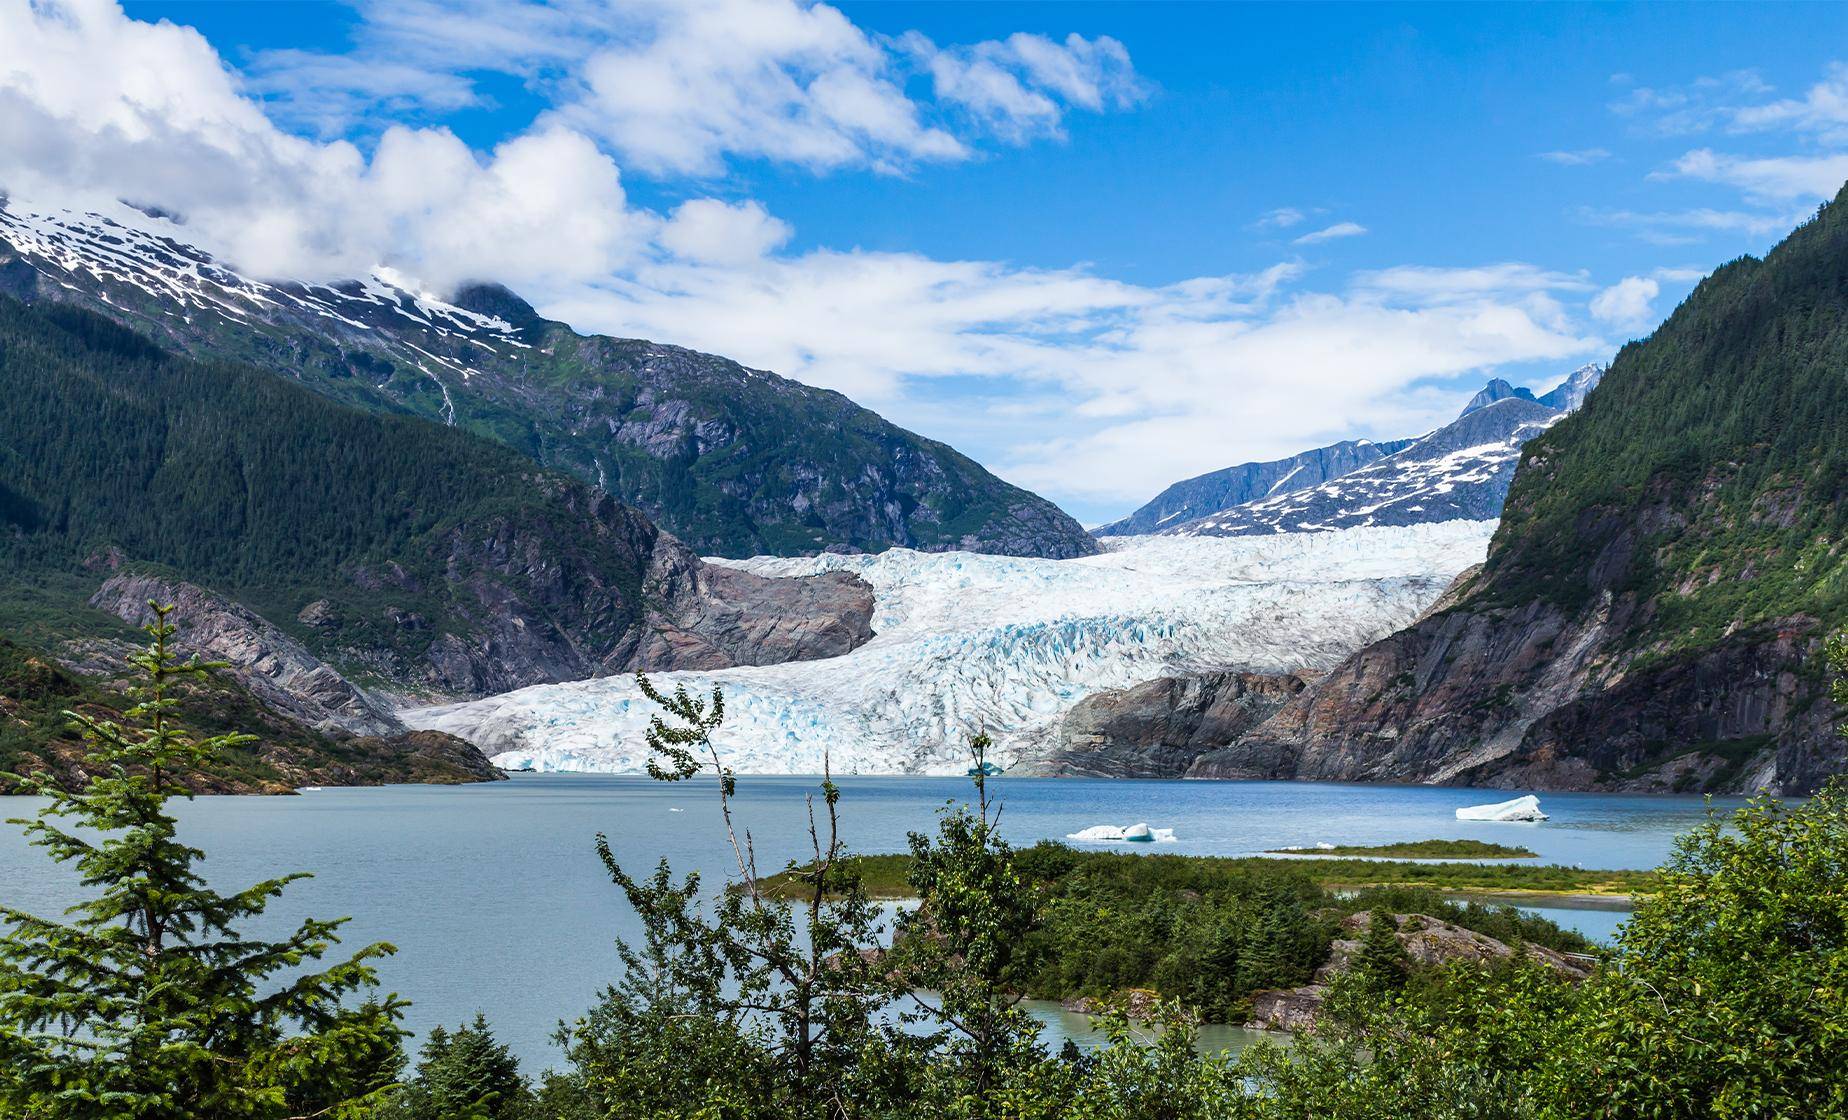
\includegraphics[width=0.7\textwidth]{figures/glaicer.jpg}
  \caption{Mendenhall Glacier, Juneau}
  \label{Fig.1}
\end{figure}
\subsection{Restatement of the Problem}
Considering the background information and restricted conditions identified in the problem statement, we are required to solve the following problems:
\begin{itemize}
  \item \textbf{Problem 1: Model Development} \\
    Develop a model to stabilize Juneau's tourism industry by optimizing income while controlling the carbon footprint, the rate of melting of glaciers. 
    and the social satisfaction. Include a sensitivity analysis to identify the most significant factors.
    
  \item \textbf{Problem 2: Revenue Allocation} \\
    Allocate the expenditures from additional revenue to areas such as infrastructure and environmental protection reasonably so that the social benifits are maxmized.
    
  \item \textbf{Problem 3: Model Adaptability} \\
    Adapt the model to other overtourism-affected tourist destinations, showing how location-specific factors influence measure importance. 
    Use the model established above to promote less-visited locations for better balance.
    
  \item \textbf{Problem 4: Memo to Tourist Council} \\
    Draft a one-page memo outlining predictions, the effects of various measures, and suggestions for optimizing outcomes.
\end{itemize}


\subsection{Our Work}
%TODO

\section{Assumption and Justification}
\begin{itemize}
  \item \textbf{Assumption1:} The data we use are accurate and valid. 
  \item \textbf{Justification1:} Our data is collected from the Juneau government and some other official websites and research papers. 
  It is reasonable to assume that the data are of high quality.

  \item \textbf{Assumption2:} Juneau will remain relatively stable, with no drastic environmental changes or social unrest.
  \item \textbf{Justification2:} A stable natural and social environment provides a predictable framework within which we can build model and make decisions. 
  It is important to note that this assumption does not neglect the potential impact of predictable environmental and social change.
  
  \item \textbf{Assumption3:} The touristsm, locals and the government are rational decision-makers aiming to maximize their own utility and possessing complete logical reasoning abilities.% 因为用了博弈论模型,加上理性人假设
  \item \textbf{Justification3:} This assumption is well-grounded in economic theory. Tourists typically make travel decisions based on cost-benefit analysis\cite{crouch2004determinants}, 
  and local residents engage in tourism-related activities to maximize their benefits\cite{ap1992residents}.
\end{itemize}

\section{Notations}
\begin{table}[H]
  \caption{\textbf{Notations}}
  \centering
  \begin{threeparttable}
    \begin{tabular}{ccc}
      \toprule
        Symbol\tnote{1} & Definition & Unit \\
      \midrule
        $V_t$ & number of tourists & million \\ 
        $C_t$ & carbon emissions per tourist & ton/person \\
        $F_t$ & amount of waste produced per tourist & tons/person \\

        $T_p$ & net income from tourism & billion\$ \\
        $T_h$ & hotel tax rate & \% \\
        $T_v$ & tourist fees & \$/person \\

        $E_t$ & comprehensive indicators of environmental quality(0-100) & / \\
        $G_t$ & rate of retreat of glaciers & meter/year \\

        $S_t$ & the score of social stability(0-10) & / \\ 
        $K_t$ & investment in infrastructure & / \\

        $M_t$ & extent of melting of glaciers & / \\
        $E_G$ & investment in environment protection of scenery spots & billion\$/year \\
        \bottomrule
    \end{tabular}
    \begin{tablenotes}
    \footnotesize
      \item[1] The symbols with subscript t represent the indicators of year t.
    \end{tablenotes}
  \end{threeparttable}
\end{table}

\section{Data Preparation}
\subsection{Data Collection}
\begin{table}[H]
  \caption{\textbf{Data Websites}} 
  \centering
  \begin{tabular}{cc}
    \toprule 
      Database Name & Database Website \\
    \midrule
      Juneau & \href{https://juneau.org}{https://juneau.org} \\ 
      JEDC & \href{https://www.jedc.org}{https://www.jedc.org} \\
      EJSCREEN & \href{https://gaftp.epa.gov/ejscreen/}{https://gaftp.epa.gov/ejscreen/} \\ 
      AntarcticGlaciers & \href{https://www.antarcticglaciers.org}{https://www.antarcticglaciers.org} \\
      GHGRP & \href{https://www.epa.gov/ghgreporting}{https://www.epa.gov/ghgreporting} \\
    \bottomrule
  \end{tabular}
\end{table}

\subsection{Data Preprocessing}

\section{Dynamic Management Model of Sustainable Tourism Based on Tripartite Game (DMSTM)}
% The overall structure of the model is shown in Fig.X. 需要架构图
We take the effect of the number of tourist $V_t$, the quality of environment $E_t$, 
the retreat of glaciers $G_t$, the stability of society $S$ into consideration , 
and build a game theory based model, DMSTM, to achieve the multi-objective optimization.
DMSTM aims to maxmize the net income from toruism while minizing the carbon footprint,
garbage generating and glacial recession, as well as keep the pressure on infrastructure within some limits,
to provide better decision-making advice.
In order to develop this model, we first need to calibrate the parameters to estimate 
the independent variables $V_t, E_t, G_t, S$ mentioned above.

\subsection{Parameters Calibration}

\subsubsection{The Number of Tourist}
The number of tourist is affected by many factors, such as the number of tourist in the last few years, 
the quality of environment, the construction of infrastructure... To predict the chagne of number of tourist,
we use multiple linear regression method

\begin{equation}
  \frac{\Delta V_t}{V_t} = \left[\left(\frac{a_{a_e}\cdot E}{E+\theta_e} + \frac{a_{a_k}\cdot K}{K+\theta_k} \right) - \beta\cdot(T_h+T_v) - \gamma\cdot(C_t+F_t) - \lambda\cdot M_t \right] \cdot e^{-e_{pdm} \cdot pdm \cdot (1 + dpdm) \cdot (1 - dmdm)}
\end{equation}

\begin{equation}
  \Delta V_t = V_{t+1} - V_t
\end{equation}

where $a_{a_e}, a_{a_k}, \beta, \gamma, \lambda$ are the parameters to fit, and they represent 
the coefficient of the environment and infrastructure attraction, the coefficient of the tax and expense restraint,
negative feedback coefficient of environmental pressure and the sensitivity coefficient of glacier melting, respectively.
While $\theta_E$ and $\theta_K$ are the saturation thresholds of environmental quality and infrastructure investment.

It is worthwhile to note that we consider the effect of epidemic specially in the exponent part of the formula, 
which will only come into effect when the year used is between 2020 to 2022, so that our predict to the number of 
visitors will be more accurate.

\subsubsection{The Environmental Quality}
The Environmental quality is impacted negatively by the carbon footprint, waste emissions, glacial retreating, and 
positively by the environmental quality in the past and the investment in environment protection. With this
insight, we build a dynamic equation to predict the environmental quality

\begin{equation}
  E_{t+1} = E_t + r_E \cdot E_t \left(1 - \frac{E}{E_{\text{max}}}\right) - \gamma_C \cdot C_t - \gamma_F \cdot F_t - \gamma_G \cdot G_t + \eta \cdot E_G
\end{equation}

where $r_E$ is the rate of self-healing of the environment, while $\gamma_C, \gamma_F, \gamma_G$ are the coefficient of 
environmental damage caused by carbon emissions, waste generating and glacial retreat. $\eta$ is the restoration efficiency of 
environmental protection investment, and $E_{max} = 100$ is the upper limit of environmental quality.

Given the complexity of this equation, we use nonlinear least squares method to fit the parameters with 
a reasonable restraint that all parameters are positive.

% In order to describe our process of fitting the parameters to predict the environmental quality more clearly,
% we draw the flowchart Figure X below

\subsubsection{Glacial Retreat}
In our model, the rate of glacial retreat is determined by this rate in the past, the carbon emissions and the number of visitors.
So we construct a linear model

\begin{equation}
  G_t = A \cdot C_t + \mu \cdot V_t + G_0
\end{equation}

and use linear regression to fit the parameters. The intercept $G_0$ is fitted as the value in reference paper, 
while $A$ and $\mu$ are the parameters to learn.

\subsubsection{Social Stability}
We create a score between 0 and 10 to evaluate the social stability, whose basis is mainly from 
the historical social stability score, the amount of tourists, the environmental quality and the extend of glacial retreat.
Therefore, we construct a regression model with constraint

\begin{equation}
  S_t = max\left(0, S_{\text{base}} - \alpha_{v_t} \cdot V_t + \alpha_{E_t} \cdot E_t - \alpha_{M_t} \cdot M_t\right)
\end{equation}

where $S_{\text{base}}$ is a benchmark score, while $\alpha_{v_t}, \alpha_{E_t}, \alpha_{M_t}$ are the parameters to fit 
with elastic network regression.

\subsection{Multi-Objective Optimization}
In multi-objective optimization problem, there are a number of conflicting objective functions. In this case, 
single objective optimization usually can't meet all the requirements, so we need to introduce multi-objective 
optimization method to find a set of compromise solutions to make balance between different goals.

Specialize to this problem, we build a tripartite game based dynamic management model, DMSTM, in which 
we regard the tourists, the locals and the government as rational actors,
and consider several goals, including the net income from tourism, the amount of carbon footprint, 
the amount of waste produced and the rate of glacial retreat. 

Due to the interrelation and potential conflict of the objectives, we use the weight coefficients $w_1, w_2, w_3$ to reflect 
the importance of each objective to the overall strategy. The final objective function can be represented as 

\begin{equation}
  Max \ (w_1 \cdot T_p - w_2 \cdot (C_t + F_t + G_t) - w_3 \cdot K_{I,t})
\end{equation}

where $K_{I,t}=\frac{K_t}{K_{\text{max}}}$ represent the pressure on infrastructure.

Additionally, we add the constraints that $E_t \geq 30$ and $V_t \leq 2.0$ to ensure that
while pursuing the maximizing of tourism income, the social well-being and ecological Sustainability
are guaranteed to some extend.

As for the solution method, we use NSGA-\uppercase\expandafter{\romannumeral2} algorithm to find
\emph{Pareto Front}, which provides a set of choice of strategies for the decision makers to give consideration to
both economic benefits and social weal as well as environmental protection.
% 需要添加算法求解流程图

\subsection{Model Results and Analysis}

\subsection{Sensitivity Analysis}

\section{Social Welfare Model via Sustainable Tax Feedback}
% 需要新模型的架构图
Though DMSTM takes the social stability as a optimization objective, it does not consider the social benefits explicitly. 
In order to achieve the optimization goal of serving the best interest of the locals while maxmizing the tourism income 
and preserving the environment, we extend DMSTM such that it takes the Sustainable tax distribution and dynamic feedback mechanism
into consideration, and regards the social benefits as a optimization objective.

\subsection{Tax and Expenditure Variables}
For the sake of representing the effect of sustainable tax distribution and dynamic feedback, 
several variables about tax are introduced to extend our model:

\begin{equation}
  T_t = \alpha \cdot T_p
\end{equation}

where $T_t$ represents the \textbf{general tax revenue}, $T_p = V_t \cdot R_p (\text{net income from tourism})$, 
and $\alpha$ stands for the the overall tax rate.

As for the expenditures, social spending are divided into three parts: \textbf{the infrastructure expenditures}, 
\textbf{the environmental protection expenditures} and \textbf{the community development expenditures}, 
such that the solution is facilittated while the actual complexity is reflected:

\begin{gather}
  K_t = x_1 \cdot T_t  \\
  E_{G,t} = x_2 \cdot T_t  \\
  C_{D,t} = x_3 \cdot T_t 
\end{gather}

where $x_1, x_2, x_3$ represent the rate of each expenditure, which meet the constraint $x_1 + x_2 + x_3 = 1$.

These three parameters also reflect the feedback mechanism. Increasing $x_1$ will increase tourist attraction, 
but at the cost of increased carbon emissions and environmental costs; increasing $x_2$ can slow down the retreat
of glaciers($G_t \downarrow$) and improve the environmental quality($E_t \uparrow$); increasing $x_3$ has the effect of
enhance the social stability($S_t\uparrow$) such that the current limit policy can be avoided.

\subsection{Social Benefits Target}
Base on the allocation of the tax, we propose a novel model to maxmize the social welfare:

\begin{equation}
  E_{\text{social}} = \beta_1 \ln(1+K_t) + \beta_2 \ln(1 + E_{G,t}) + \beta_3 \ln(1 + C_{D,t})
\end{equation}

where $\beta_1, \beta_2, \beta_3$ are the efficiency weight of the fields and should be setted by the decision-maker.
With our analysis, the recommanded values are $\beta_1=0.3, \beta_2=0.4, \beta_3=0.4$

While each of these three expenditures has its own rate, the overall balance is also important. After observing the 
these three kind of expenditures of Juneau government from 2014 to 2022, we decide to introduce several 
dynamic management rules to ensure their relative balance:

\begin{equation}
\begin{aligned}
  & x_3\uparrow & \text{if } S_t < 5 \\
  & x_2\uparrow & \text{if } E_t < 60  
\end{aligned}
\end{equation}

\subsection{Multi-Objective Optimization Modification}
After taking the social welfare into optimizing target, now the target function of extended DMSTM becomes 

\begin{align}
\left\{
  \begin{aligned}
    & Maximize \quad w_1 \cdot T_p - w_2 \cdot (C_t + F_t + G_t) - w_3 \cdot K_t \\ 
    & Maximize \quad E_{\text{social}}
  \end{aligned}
\right.
\end{align}

Because we only add a new optimization objective, the original constraints such as $x_1+x_2+x_3=1, x_1>0,x_2>0,x_3>0$ 
remains unchanged. And we still use NSGA-\uppercase\expandafter{\romannumeral2} algorithm to find
\emph{Pareto Front} to balance economic, environmental, cost and social effect.

\section{Adapt Extended DMSTM to Franz Josef Glacier}
\subsection{The Situation of Overtourism in Franz Josef Glacier}
Franz Josef Glacier, located in Westland Tai Poutini National Park on the West Coast of New Zealand's South Island, 
is a 12-kilometer-long temperate maritime glacier. Franz Josef glacier is the one of the most publicly-accessible glaciers in New Zealand,
and among the most accessible in the world -- until recently, there was easy walking access directly to the glacier termini. 
Consequently for over a century they have been a significant tourist attraction\cite{wilson2013west}

Today the Franz Josef glacier area is the third-most-visited tourist spot in New Zealand, 
and one of the main tourist attractions on the West Coast. It had around 250,000 visitors a year in 2008, 
increasing to 700,000 a year (500,000 overnight) in 2017.

However, after 2008 this glacier entered a very rapid phase of retreat, shrinking by 1.5 km between 2008 and 2017.
It is now once again 3 km shorter than it was 100 years ago. Based on these patterns, 
Franz Josef Glacier is predicted to retreat 5 kilometres (3.1 mi) and lose 38\% of its mass by 2100 in a mid-range scenario of warming\cite{anderson2008response}

Thus it is clear to see that Franz Josef Glacier faces the challenges similar to Juneau, Alaska, where overtourism 
impact the environment greatly. Rising visitor numbers driven by adeventure tourism and glacier hikes have accelerated cie melt
due to human activity and carbon footprint, while overwhelming local resources.

\subsection{Haast As Secondary Scenic Spot}
Haast is strategically positioned as a complementary destination to Franz Josef Glacier due to its geographic proximity, ecological diversity, and historical ties.
Located along the Haast Pass—a vital route connecting Franz Josef Glacier to Wanaka—it offers contrasting landscapes like rainforests, waterfalls, and glacial-fed attractions, enriching the region's tourism portfolio.
Its role as part of the Te Wahipounamu World Heritage Area and shared heritage with explorer Julius von Haast further strengthen its cultural relevance.

By integrating Haast into tourism circuits, it effectively diverts visitor traffic from Franz Josef Glacier, mitigating overtourism impacts such as glacial degradation and infrastructure strain.
This redistribution fosters sustainable tourism: visitors engage in low-impact activities, such as hiking, wildlife viewing, while supporting local economies. 
Ultimately, Haast enhances regional resilience, balancing conservation with visitor demand and preserving the West Coast's ecological integrity.

With this consideration in mind, we further divide the tourist amount $V_t$ into $V_{t,main}$ and $V_{t,sub}$, where $V_{t,main}$ represents the number of tourists 
in the main scenery spot, Franz Josef Glacier; while $V_{t,sub}$ represents the number of tourists in complementary scenery spot, Haast.
And we use a current division factor $\phi_t$ to control the attraction of complementary destination by specific policies such that

\begin{align}
  & V_{t,main} = V_t \cdot (1 - \phi_t) \\
  & V_{t,sub} = V_t \cdot \phi_t
\end{align}

\subsection{Model Indicators}
To model the scenic spot thoroughly without losing generalities, four indicators are introduced.
For these indicators, the higher the value, the greater the weight.
% 换成一张图,说明这些indicators

\begin{table}[H]
  \caption{\textbf{Indicators}} 
  \centering
  \begin{tabular}{ccc}
    \toprule 
      Indicator & Meaning & Range \\
    \midrule
      $I_e$ & indicator of environmental vulnerability & $[0, 1]$ \\
      $I_c$ & indicator of the value of cultural heritage & $[0, 1]$ \\
      $I_i$ & indicator of infrastructure pressure & $[0, 1]$ \\
      $I_d$ & tourism as a percentage of GDP & $[0, 1]$ \\
    \bottomrule
  \end{tabular}
\end{table}

\subsection{Dynamic Formula Design}
Similar to the dynamic system modeled by DMSTM, we design the formulas to describe the amount of tourists, 
the environmental quality and the economic income. But now the indicators $I_e, I_c, I_i, I_d$ are introduced
for better adaptability. In theory, our further extended DMSTM can not only apply to Franz Josef Glacier
as the main destination and Haast as the complementary destination, but any other destinations impacted by 
overtourism or requiring promotion to deal with the problem of lacking tourists, as long as necessary data are provided.

Current division feedback and geographical attributes feedback are introduced to construct our dynamic tourists amount predicting formula:

\begin{gather}
  V_t = \alpha \cdot \left(\frac{E_t}{E_t + \theta_E} + \frac{K_t}{K_t + \theta_K} \right) - \beta \cdot (T_h + T_v)
  - \gamma \cdot (C_t + G_t) + \lambda \cdot \phi_t \cdot (1 - I_c) \\
  \lambda = 0.15 \cdot (1 + I_d)
\end{gather}

where $\lambda$ represent the coefficient of attraction of the complementary destination. The higher the economic dependence is,
this coefficient is larger.

Similarly, we introduce other indicators into the formulas of environmental quality, glacial retreat and economic income:

\begin{gather}
  E_{t+1} = E_t + r_E \cdot E_t \left(1 - \frac{E_t}{E_{max}}\right) - \gamma_C \cdot (C_{t,main} + C_{t,sub}) - \gamma_G \cdot G_t \cdot I_e + \eta \cdot K_t \\
  G_t = G_0 \cdot \exp \left(\frac{\epsilon \cdot V_{t,main}}{1+\zeta \cdot K_t}\right) \\
  T_p = p_{main} \cdot V_{t,main} \cdot I_d + p_{sub} \cdot V_{t,sub} \cdot (1 - I_d) - c_{eco} \cdot K_t
\end{gather}

where $\zeta$ is the coefficient of environmental investment to inhibit the retreat, while 
$p_{main}$ and $p_{sub}$ are the consumption per person in main and complementary destination, respectively.

\subsection{Apply Multi-Objective Optimization Model to Franz Josef Glacier}
Since we are generalizing our DMSTM to adapt to other scenic spots, the final multi-objective optimization model
also needs some modifications. To be more specific, four indicators are intergrated into the objective function dynamically.

\begin{gather}
  Maximize \quad w_1\cdot T_p - w_2 \cdot (C_t + G_t \cdot I_e) - w_3 \cdot (1 - S_t) \\ 
  w_1 = 0.4 + 0.2I_d \\
  w_2 = 0.3 + 0.2I_e \\
  w_3 = 0.3 - 0.1I_e
\end{gather}

Here, $w_1, w_2, w_3$ are determined through linear regression to assign the weight dynamically based on local circumsstances.
And these coefficient are learnt with the data of Franz Josef Glacier and Hasst. 

After determining these formulas, we use the statistics from 2018 to 2023, including the number of tourists, the greenhouse gas, 
the infrastructure investment and Franz Josef Glacier, to fit the parameters and get the \emph{Pareto Front} solution sets, which
are shown in the solution set table:

\begin{table}[H]
  \caption{Solution Sets}    
  \centering
  \begin{tabular}{ccccc}
    \toprule
    Strategy & $\phi_t$ & $K_t$ (billion) & $T_p$ (billion) & $G_t$ (m/year) \\
    \midrule
    economy first & 0.25 & 0.30 & 0.62 & 1.18 \\
    ecology first & 0.12 & 0.80 & 0.45 & 0.95 \\
    balanced & 0.18 & 0.60 & 0.53 & 1.05 \\
    \bottomrule
  \end{tabular}
\end{table}

\section{Model Evaluation}
\subsection{Strengths}
\begin{itemize}
 \item \textbf{Comprehensive Consideration} \\
 Our DMSTM and its extended versions, take multiple factors into account simultaneously . 
 For example, in DMSTM, we consider the number of tourists, environmental quality, glacial retreat, and social stability. 
 This holistic approach provides a more accurate representation of the complex relationships within the tourism system, 
 empowering better decision-making. It allows for a balanced assessment of economic, environmental, and social impacts, 
 which is crucial for sustainable tourism development.
 \item \textbf{Data-Driven and Rigorous Parameter Calibration} \\
 We collect data from reliable sources such as government websites and research papers.
 The parameters in our models are calibrated using appropriate statistical methods, like multiple linear regression and elastic network regression method.
 This data-driven approach ensures that the models are based on real-world data, enhancing their accuracy and reliability.
 \item \textbf{Multi-Objective Optimization} \\
 By using multi-objective optimization methods like the NSGA-\uppercase\expandafter{\romannumeral2} algorithm,
 we are able to find sets of \emph{Pareto-optimal} solutions. This approach is better than single-objective optimization, 
 as it addresses the conflicting goals in tourism management, such as maximizing tourism income while minimizing environmental damage and maintaining social stability.
 \item \textbf{Adaptability} \\
 The models are adaptable to different tourist destinations.
 We demonstrated this ability by applying the extended DMSTM to Franz Josef Glacier in New Zealand.
 With location-specific indicators and dynamic formulas introduced, the model can be customized to fit the unique characteristics of various regions affected by overtourism or in need of tourism promotion.
 This adaptability increases the model's practical value.
\end{itemize}

\subsection{Weeknesses}
\begin{itemize}
 \item \textbf{Simplifying Assumptions} \\
 Although our assumptions are reasonable, they do simplify the real-world situation to some extent.
 For instance, assuming that tourists, locals, and the government are perfectly rational decision-makers with complete information may not hold true in reality.
 In practice, decision-makers will be influenced by emotions, limited knowledge, and external factors not accounted for in the model.
 However, these assumptions are common in economic-based models and do not severely undermine the overall validity of the results.
 \item \textbf{Model Complexity} \\
 With limited time to develop and optimize our models, they are relatively complex, with multiple equations and parameters.
 This complexity may make it challenging for some stakeholders, such as local community members or small-scale tourism operators,
 to fully understand and interpret the results.
 While efforts have been made to simplify the presentation of findings, 
 further work should be done to make the models more accessible without sacrificing their accuracy.
\end{itemize}

\section{Conclusions}

% \subsection{How to cite?}
% bibliography cite use \cite{1,2,3}

% AI cite use \AIcite{AI1,AI2,AI3}

% \begin{thebibliography}{99}
% \bibitem{1} D.~E. KNUTH   The \TeX{}book  the American
% Mathematical Society and Addison-Wesley
% Publishing Company , 1984-1986.
% \bibitem{2}Lamport, Leslie,  \LaTeX{}: `` A Document Preparation System '',
% Addison-Wesley Publishing Company, 1986.
% \bibitem{3}\url{https://www.latexstudio.net/}
% \end{thebibliography}
\bibliographystyle{unsrt}
\bibliography{mcmthesis-demo}

\begin{appendices}

\section{First appendix}

% In addition, your report must include a letter to the Chief Financial Officer (CFO) of the Goodgrant Foundation, Mr. Alpha Chiang, that describes the optimal investment strategy, your modeling approach and major results, and a brief discussion of your proposed concept of a return-on-investment (ROI). This letter should be no more than two pages in length.

% \begin{letter}{Dear, Mr. Alpha Chiang}

% \lipsum[1-2]

% \vspace{\parskip}

% Sincerely yours,

% Your friends

% \end{letter}
% Here are simulation programmes we used in our model as follow.\\

% \textbf{\textcolor[rgb]{0.98,0.00,0.00}{Input matlab source:}}
% \lstinputlisting[language=Matlab]{./code/mcmthesis-matlab1.m}

% \section{Second appendix}

% some more text \textcolor[rgb]{0.98,0.00,0.00}{\textbf{Input C++ source:}}
% \lstinputlisting[language=C++]{./code/mcmthesis-sudoku.cpp}

\end{appendices}


\AImatter

% \begin{ReportAiUse}{9}
% \bibitem{AI1}
% Bing AI\\
% Query1: write a sort algorithm\\
% Output: Sure, I can help you with that. Here is a simple implementation of the selection sort algorithm in Python:
% \begin{lstlisting}[language=python]
% def selection_sort(arr):
%     for i in range(len(arr)):
%         min_idx = i
%         for j in range(i + 1, len(arr)):
%             if arr[min_idx] > arr[j]:
%                 min_idx = j
%         arr[i], arr[min_idx] = arr[min_idx], arr[i]
%     return arr
% \end{lstlisting}
% This algorithm sorts an array by repeatedly finding the minimum element from the unsorted part of the array and putting it at the beginning. \href{https://www.geeksforgeeks.org/sorting-algorithms/}{The time complexity of this algorithm is O($n^2$)}.

% There are many other sorting algorithms available such as bubble sort, insertion sort, merge sort, quick sort, heap sort, and more. Each of these algorithms has its own advantages and disadvantages. You can learn more about them on GeeksforGeeks and Programiz.

% I hope this helps!

% \bibitem{AI2}
% OpenAl Enie (Nov 5, 2023 version, Ernie 4.0)\\
% Query1: <insert the exact wording of any subsequent input into the Al tool>\\
% Output: <insert the complete output from the second query>

% \bibitem{AI3}
% Github CoPilot (Feb 3, 2024 version)\\
% Query1: <insert the exact wording you input into the Al tool>\\
% Output: <insert the complete output fron the Al tool>

% \bibitem{AI4}
% Google Bard (Feb 2,2024 version)\\
% Query: <insert the exact wording of your query>\\
% Output: <irsert the complete output from the Al tool>

% \bibitem{AI5}
% Bing AI\\
% Query: write a FFT algorithm\\
% Output: Sure, here is a Python implementation of the Fast Fourier Transform (FFT) algorithm:
% \begin{lstlisting}[language=python]
% import numpy as np

% def fft(x):
%     n = len(x)
%     if n == 1:
%         return x
%     even = fft(x[0::2])
%     odd = fft(x[1::2])
%     T = [np.exp(-2j * np.pi * k / n) * odd[k] for k in range(n // 2)]
%     return [even[k] + T[k] for k in range(n // 2)] + [even[k] - T[k] for k in range(n // 2)]
% \end{lstlisting}
% The FFT is a widely used algorithm for computing the \textbf{Discrete Fourier Transform (DFT)} of a sequence. It reduces the number of computations needed from O(n$^2$) to O(n log n) 12. The basic idea of the FFT is to apply divide and conquer. We divide the coefficient vector of the polynomial into two vectors, recursively compute the DFT for each of them, and combine the results to compute the DFT of the complete polynomial 3.

% I hope this helps!

% \end{ReportAiUse}
%% Generate the Memorandum, if it's needed.
\memoto{The Tourist Councill of Juneau}
\memofrom{Team \# 2525570}
\memosubject{Urgent Actions to Balance Tourism and Glaicer Preservation}
\memodate{\today}
\memologo{COMAP}
\begin{memo}[Memorandum]
  We are Juneau sustainable tourism model developers. Base on our modelings and findings, we would like
  to inform you our prediction, the effects of different measures and our suggestions on optimizing the outcome.

  % 数据换成我们跑的
  Juneau's glaciers are experiencing accelerated melting due to unsustainable tourism practices nowadays. 
  Our analysis indicated that without immediate intervention, annual glacier retreat rates will increase by 15\%
  over the next five years, severely damaging both ecological integrity and long-term tourism stability. 
  Current visitor numbers (2,300+ daily) exceed the glacial ecosystem's carrying capacity by 35\%, directly contributing to irreversible environmental damage. 
  Additionally, resident satisfaction scores have fallen to 4.2/10, signaling growing community opposition to unchecked tourism.

  In order to change this deteriorating situation, some immediate actions must be taken:
  \begin{enumerate}
    \item \textbf{Implement vistor capacity controls}, restrict daily visitors to 1,500 throught a reservation system to reduce the glacial stress by 23\%.
    \item \textbf{Launch the glacier sustainability fund}, collect the environmental tax and use over 70\% of them directly for glacier restoration.
    \item \textbf{Strengthen community engagement} by allocating 30\% of tourism revenue to local infrastructure construction, aiming to cut $\text{CO}_\text{2}$ emission by 25\% by 2026s.
  \end{enumerate}

  Besides, for the long-term strategic plan, we also recommand deploy IoT sensors across critical glacial zones to track melt rates and implement real-time monitoring, as well as
  developing state-of-the-art algorithm to recalibrate visitor caps dynamically based on real-time environmental data.

  After adapting these measures, the annual glacial retreat should be reduced from 1.2 to 0.8 meters by 2026, while the toursim revenue can maintain above \$5.5 milllion annually with
  low-impact tourism models, and the transparent revenue sharing will restore community trust.

  As grim as the situation may be, we are confident in your decision-makings, and know that the sustainable toursim pattern will be established
  with your rational measures.
\end{memo}

\end{document}
%% 
%% This work consists of these files mcmthesis.dtx,
%%                                   figures/ and
%%                                   code/,
%% and the derived files             mcmthesis.cls,
%%                                   mcmthesis-demo.tex,
%%                                   README,
%%                                   LICENSE,
%%                                   mcmthesis.pdf and
%%                                   mcmthesis-demo.pdf.
%%
%% End of file `mcmthesis-demo.tex'.

